% ============================================================
%  CHAPITRE 2 — ANALYSE ET SPÉCIFICATION DES BESOINS
% ============================================================
\chapter{Analyse et spécification des besoins}

\vspace{-0.5cm}
\begin{tcolorbox}[colback=lightgray, colframe=primaryblue, title=\textbf{Plan du chapitre}, fonttitle=\bfseries]
  \begin{enumerate}[leftmargin=*, label=\arabic*.]
    \item Spécification des besoins \dotfill \pageref{sec:besoins}
    \item Analyse globale \dotfill \pageref{sec:analyse_globale}
    \item Élaboration du Backlog produit \dotfill \pageref{sec:backlog}
    \item Planification du travail \dotfill \pageref{sec:planification}
    \item Architecture de la solution \dotfill \pageref{sec:architecture}
    \item Choix techniques \dotfill \pageref{sec:choix_techniques}
    \item Mise en place de la solution DevOps \dotfill \pageref{sec:devops}
  \end{enumerate}
\end{tcolorbox}

% ─────────────────────────────────────────────────────────
\section*{Introduction}
% ─────────────────────────────────────────────────────────

Ce chapitre a pour objectif de présenter l'ensemble des acteurs impliqués dans la plateforme
SmartPM ainsi que les besoins fonctionnels et non fonctionnels qui lui sont associés. Cette
première étape permettra de structurer le backlog produit et de garantir une compréhension
précise et partagée des exigences du projet.

Dans un second temps, une analyse globale sera réalisée à travers des diagrammes UML~\cite{uml} afin
de décrire l'architecture à adopter pour la solution proposée. Enfin, le chapitre se conclura
par la planification des sprints, illustrant l'organisation et le déroulement du développement.


% ─────────────────────────────────────────────────────────
\section{Spécification des besoins}
\label{sec:besoins}
% ─────────────────────────────────────────────────────────

\subsection{Identification des acteurs}

Afin de bien comprendre le périmètre et les interactions de la plateforme SmartPM, nous
identifions dans cette section les différents acteurs qui interagissent avec le système.
SmartPM comporte trois rôles d'utilisateurs internes principaux :

\subsubsection{Administrateur (Admin)}

L'administrateur est le super-utilisateur de la plateforme. Il dispose d'un accès complet
à l'ensemble des fonctionnalités de configuration et de supervision. Son rôle principal est
de gérer les comptes utilisateurs, d'assigner les rôles, de consulter les journaux d'audit
et de maintenir la cohérence des données du système.

\subsubsection{Manager (Chef de projet)}

Le Manager est l'utilisateur central de SmartPM. Il est responsable de la création et de
la supervision des projets qui lui sont confiés. Il dispose d'un tableau de bord dédié lui
offrant une vision globale de l'avancement de ses projets, de la charge de son équipe et des
métriques clés. Il peut créer des projets via un wizard multi-étapes, affecter des membres
à des tâches et générer des rapports grâce à l'intelligence artificielle intégrée.

\subsubsection{Member (Membre d'équipe)}

Le Member est un collaborateur affecté à un ou plusieurs projets. Il dispose d'un tableau
de bord personnel lui présentant ses tâches en cours, ses certifications à valider et ses
revues en attente. Il peut soumettre des revues de tâches (dans le respect de la règle
Author~$\neq$~Reviewer) et utiliser l'assistant IA pour obtenir de l'aide sur ses tâches.

\vspace{0.3cm}

\begin{figure}[H]
  \centering
  \begin{tikzpicture}[
      scale=1.1, transform shape,
      actor/.style={draw, rounded corners=8pt, thick, align=center, minimum width=3.8cm, minimum height=2cm},
      admin/.style={actor, draw=red!70, fill=red!5, text=red!80!black},
      manager/.style={actor, draw=primaryblue!80, fill=primaryblue!5, text=primaryblue!80!black},
      member/.style={actor, draw=successgreen!80, fill=successgreen!5, text=successgreen!80!black},
      platform/.style={draw=darkgray, very thick, rounded corners=12pt, fill=gray!5, minimum width=4cm, minimum height=2.5cm, align=center, font=\Large\bfseries\color{primaryblue}}
  ]
      % Acteurs
      \node[admin] (admin) at (-5, 3) {\LARGE\faUserShield\\[0.1cm]\normalsize\textbf{Administrateur}\\[0.1cm]\scriptsize Supervision globale};
      \node[manager] (manager) at (-5, 0) {\LARGE\faUserTie\\[0.1cm]\normalsize\textbf{Manager}\\[0.1cm]\scriptsize Gestion des projets};
      \node[member] (member) at (-5, -3) {\LARGE\faUser\\[0.1cm]\normalsize\textbf{Member}\\[0.1cm]\scriptsize R\'ealisation des t\^aches};

      % Plateforme
      \node[platform] (sys) at (0, 0) {\faRocket\\[0.1cm] SmartPM};

      % Lignes
      \draw[very thick, -stealth, darkgray] (admin) -| (sys.north);
      \draw[very thick, -stealth, darkgray] (manager) -- (sys);
      \draw[very thick, -stealth, darkgray] (member) -| (sys.south);
  \end{tikzpicture}
  \caption{Sch\'ema des acteurs de la plateforme SmartPM}
  \label{fig:acteurs}
\end{figure}

\subsection{Identification des besoins fonctionnels}

La plateforme SmartPM doit répondre aux besoins fonctionnels suivants, répartis par acteur :

\vspace{0.3cm}
\textbf{L'Administrateur doit pouvoir :}
\begin{itemize}
  \item Créer, modifier, désactiver et supprimer des comptes utilisateurs
  \item Assigner et modifier les rôles des utilisateurs (Admin / Manager / Member)
  \item Consulter les journaux d'audit (actions, connexions, modifications)
  \item Réinitialiser les mots de passe des utilisateurs
  \item Superviser les métriques globales de la plateforme (Prometheus/Grafana)
\end{itemize}

\vspace{0.3cm}
\textbf{Le Manager doit pouvoir :}
\begin{itemize}
  \item Créer un projet via un wizard multi-étapes (nom, description, dates, équipe)
  \item Gérer la hiérarchie des tâches : Activités~$\rightarrow$ Sous-Activités~$\rightarrow$ Tâches
  \item Affecter des tâches à des membres et définir leurs échéances et priorités
  \item Suivre l'avancement global du projet via un tableau de bord dédié
  \item Utiliser l'IA pour simuler l'avancement du projet et générer des rapports
  \item Consulter les certifications et revues de son équipe
\end{itemize}

\vspace{0.3cm}
\textbf{Le Member doit pouvoir :}
\begin{itemize}
  \item Consulter ses tâches assignées et leur statut
  \item Mettre à jour le statut de ses tâches (TODO / IN\_PROGRESS / IN\_REVIEW / DONE)
  \item Soumettre des revues sur des tâches (Author~$\neq$~Reviewer)
  \item Valider les certifications correspondant à sa phase courante (HLR/LLR/CODE/LLT/HLT)
  \item Commenter des tâches et recevoir des notifications en temps réel
  \item Interagir avec le chatbot IA pour obtenir des réponses contextuelles
\end{itemize}

\subsection{Identification des besoins non fonctionnels}

L'efficacité de SmartPM repose non seulement sur ses fonctionnalités, mais également sur
des aspects non fonctionnels garantissant une expérience utilisateur optimale et la fiabilité
du système.

\begin{itemize}
  \item \textbf{Sécurité :} Authentification JWT avec expiration configurable, OAuth2 via Google
  et GitHub, protection CORS stricte, en-têtes de sécurité HTTP via Helmet, rate limiting
  (100 requêtes/minute par IP) contre les attaques DDoS et brute-force.

  \item \textbf{Performance :} Temps de réponse API inférieur à 2 secondes pour les opérations
  courantes, réponse du chatbot IA en moins d'une seconde grâce à Groq (streaming SSE).

  \item \textbf{Disponibilité :} Architecture Kubernetes avec 2 réplicas pour le backend et
  le frontend, garantissant une haute disponibilité et une tolérance aux pannes.

  \item \textbf{Scalabilité :} Architecture modulaire NestJS permettant l'ajout de nouveaux
  modules sans impact sur les fonctionnalités existantes. Kubernetes permet le scaling horizontal
  automatique selon la charge.

  \item \textbf{Maintenabilité :} Code TypeScript strict, architecture en couches (Controller /
  Service / Repository), documentation API auto-générée via Swagger.

  \item \textbf{Observabilité :} Monitoring en temps réel via Prometheus (métriques API,
  latence, erreurs) et Grafana (dashboards visuels). Backup automatique de la base de données
  MongoDB Atlas.
\end{itemize}


% ─────────────────────────────────────────────────────────
\section{Analyse globale}
\label{sec:analyse_globale}
% ─────────────────────────────────────────────────────────

\subsection{Diagramme de cas d'utilisation global}

La figure~\ref{fig:use_case_global} présente le diagramme de cas d'utilisation global de la
plateforme SmartPM, illustrant les interactions entre les trois acteurs principaux et les
fonctionnalités du système.

\begin{figure}[H]
  \centering
  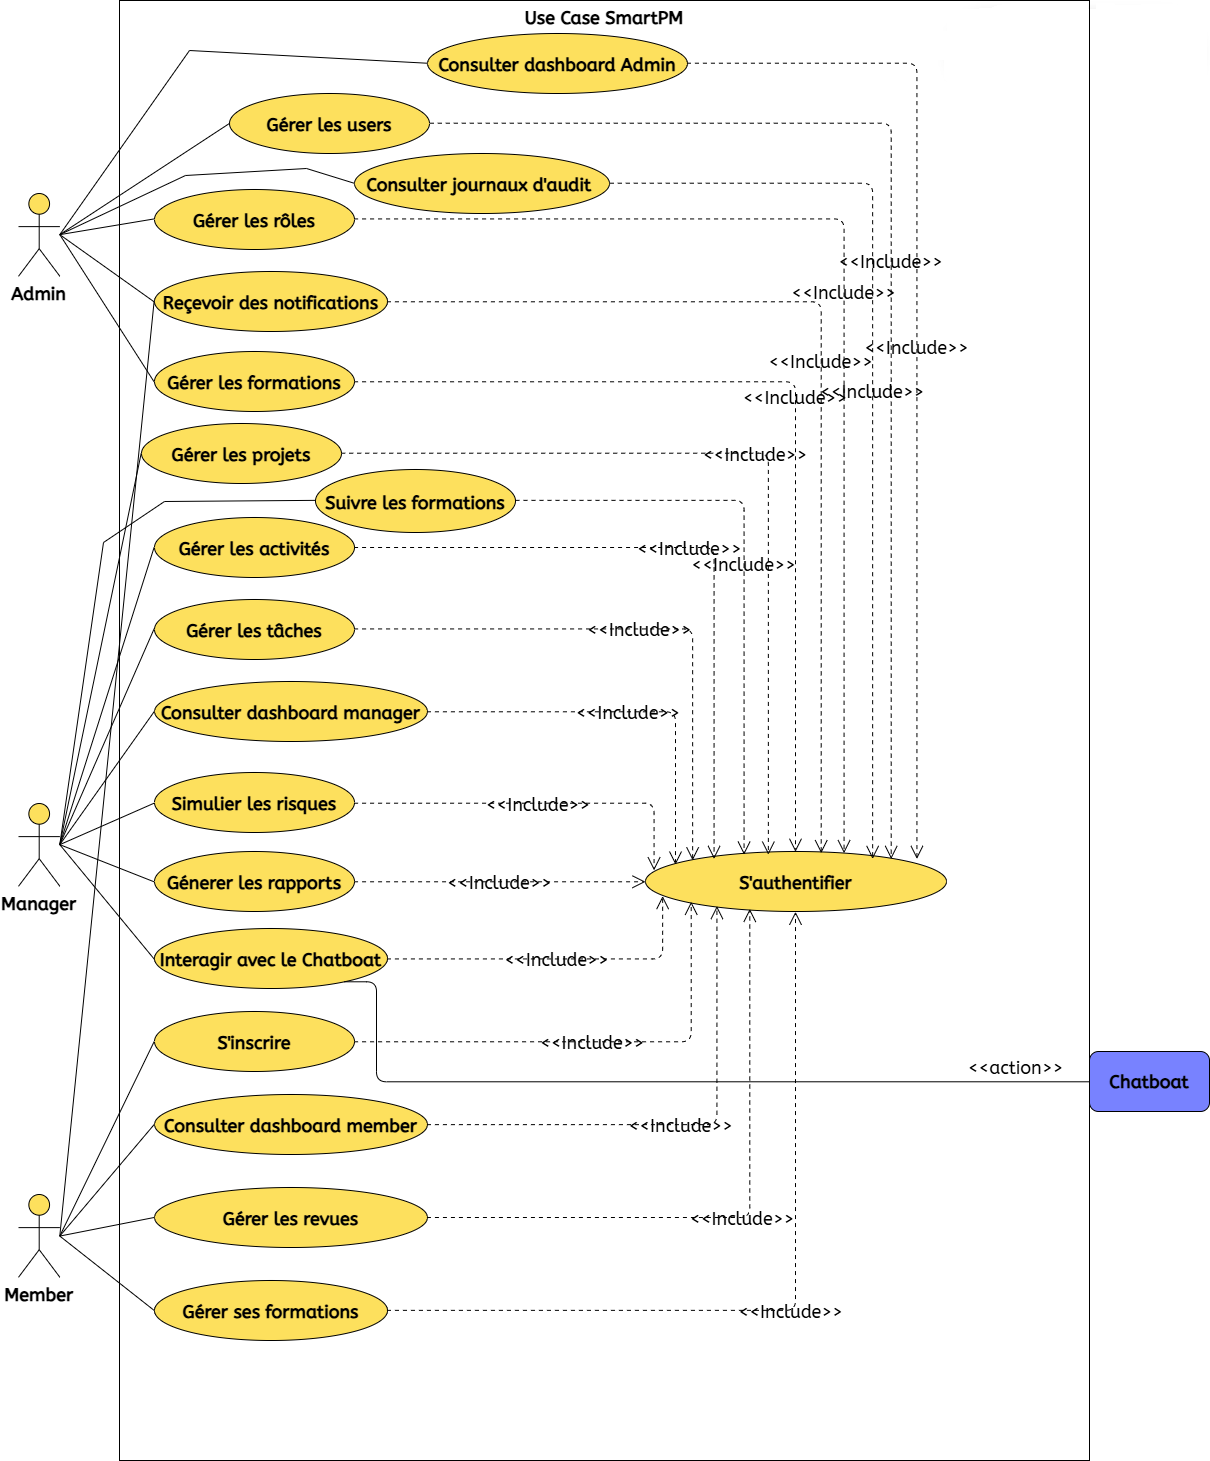
\includegraphics[width=\textwidth]{images/diagram-usecase.png}
  \caption{Diagramme de cas d'utilisation global de SmartPM}
  \label{fig:use_case_global}
\end{figure}

\subsection{Diagramme de classes global}

La figure~\ref{fig:class_global} présente le diagramme de classes global de SmartPM,
illustrant la structure des principales entités du système et leurs relations.

\begin{figure}[H]
  \centering
  \includegraphics[width=\textwidth]{images/diagram-classes.jpg}
  \caption{Diagramme de classes global de SmartPM}
  \label{fig:class_global}
\end{figure}


% ─────────────────────────────────────────────────────────
\section{Élaboration du Backlog produit}
\label{sec:backlog}
% ─────────────────────────────────────────────────────────

Dans Scrum, le Backlog produit regroupe l'ensemble des exigences liées au produit,
transformées en User Stories. Chaque User Story décrit une fonctionnalité du point de vue
de l'utilisateur et est associée à une priorité et une charge estimée.

Notre tableau~\ref{tab:backlog} est caractérisé par les champs suivants :
\begin{itemize}
  \item \textbf{ID} : Identifiant unique auto-incrémenté
  \item \textbf{User Story} : Scénario décrivant la valeur ajoutée de la fonctionnalité
  \item \textbf{Priorité} : Valeur numérique (1 = haute, 4 = basse)
  \item \textbf{Charge} : Estimation en jours de développement
\end{itemize}

\begin{longtable}{|c|p{7cm}|c|c|}
  \caption{Backlog produit global de SmartPM}
  \label{tab:backlog} \\
  \hline
  \rowcolor{tablehead}
  \textcolor{white}{\textbf{ID}} &
  \textcolor{white}{\textbf{User Story}} &
  \textcolor{white}{\textbf{Priorité}} &
  \textcolor{white}{\textbf{Charge (j)}} \\
  \hline
  \endfirsthead
  \multicolumn{4}{c}{\textit{Suite du Backlog produit}} \\
  \hline
  \textbf{ID} & \textbf{User Story} & \textbf{Priorité} & \textbf{Charge} \\
  \hline
  \endhead
  \hline
  \endfoot

  % Sprint 1
  \multicolumn{4}{|c|}{\cellcolor{primaryblue!20}\textbf{Sprint 1 — Authentification \& Gestion des utilisateurs}} \\
  \hline
  US01 & En tant qu'utilisateur, je peux m'authentifier avec email/mot de passe via JWT & 1 & 4 \\
  \hline
  US02 & En tant qu'utilisateur, je peux me connecter via Google OAuth2 & 2 & 3 \\
  \hline
  US03 & En tant qu'utilisateur, je peux me connecter via GitHub OAuth2 & 2 & 2 \\
  \hline
  US04 & En tant qu'Admin, je peux créer, modifier et désactiver des comptes utilisateurs & 1 & 3 \\
  \hline
  US05 & En tant qu'Admin, je peux assigner/modifier les rôles des utilisateurs & 1 & 2 \\
  \hline
  US06 & En tant qu'Admin, je consulte les journaux d'audit (connexions, actions) & 3 & 2 \\
  \hline

  % Sprint 2
  \multicolumn{4}{|c|}{\cellcolor{primaryblue!20}\textbf{Sprint 2 — Gestion des projets, activités et tâches}} \\
  \hline
  US07 & En tant que Manager, je crée un projet via un wizard multi-étapes & 1 & 5 \\
  \hline
  US08 & En tant que Manager, je gère les activités d'un projet (CRUD) & 1 & 3 \\
  \hline
  US09 & En tant que Manager, je gère les sous-activités (CRUD) & 2 & 3 \\
  \hline
  US10 & En tant que Manager, je crée et assigne des tâches aux membres & 1 & 4 \\
  \hline
  US11 & En tant que Manager, je consulte le tableau de bord global de mes projets & 2 & 3 \\
  \hline
  US12 & En tant que Member, je consulte mon tableau de bord personnel (tâches, certif.) & 2 & 3 \\
  \hline

  % Sprint 3
  \multicolumn{4}{|c|}{\cellcolor{primaryblue!20}\textbf{Sprint 3 — Revues, certifications \& notifications}} \\
  \hline
  US13 & En tant que Member, je soumets une revue sur une tâche (Author $\neq$ Reviewer) & 1 & 4 \\
  \hline
  US14 & En tant que Member, je valide ou rejette une revue soumise par un pair & 1 & 3 \\
  \hline
  US15 & En tant que Member, je valide une certification pour une phase DO-178C & 2 & 4 \\
  \hline
  US16 & En tant qu'utilisateur, je commente une tâche (fil de discussion) & 3 & 2 \\
  \hline
  US17 & En tant qu'utilisateur, je reçois des notifications en temps réel & 3 & 3 \\
  \hline

  % Sprint 4
  \multicolumn{4}{|c|}{\cellcolor{primaryblue!20}\textbf{Sprint 4 — Intelligence artificielle \& Formations}} \\
  \hline
  US18 & En tant qu'utilisateur, j'interagis avec le chatbot AI contextuel (données live) & 1 & 5 \\
  \hline
  US19 & En tant que Manager, je simule l'avancement et les risques de mon projet via l'IA & 2 & 4 \\
  \hline
  US20 & En tant que Manager, je génère un rapport de projet automatique via l'IA & 3 & 3 \\
  \hline
  US21 & En tant qu'utilisateur, j'accède aux formations (PDF/vidéo) liées au projet & 4 & 3 \\
  \hline

  % Sprint 5
  \multicolumn{4}{|c|}{\cellcolor{primaryblue!20}\textbf{Sprint 5 — DevOps, monitoring \& sécurité}} \\
  \hline
  US22 & Le système est containerisé via Docker (3 images : frontend, backend, AI) & 1 & 3 \\
  \hline
  US23 & Le système est déployé sur Kubernetes avec haute disponibilité (6 pods) & 1 & 5 \\
  \hline
  US24 & Les métriques sont collectées par Prometheus et visualisées dans Grafana & 2 & 4 \\
  \hline
  US25 & Le système implémente Helmet, CORS strict et Rate Limiting (100 req/min) & 1 & 2 \\
  \hline
  US26 & Le backup automatique MongoDB est configuré et testé & 3 & 2 \\
  \hline
\end{longtable}


% ─────────────────────────────────────────────────────────
\section{Planification du travail}
\label{sec:planification}
% ─────────────────────────────────────────────────────────

\subsection{Répartition des sprints par release}

Le tableau~\ref{tab:sprints} présente la répartition des sprints par release, avec leur
durée et leur objectif principal.

\begin{table}[H]
  \centering
  \caption{Planification des sprints par release}
  \label{tab:sprints}
  \renewcommand{\arraystretch}{1.5}
  \begin{tabularx}{\textwidth}{|c|c|X|c|}
    \hline
    \rowcolor{tablehead}
    \textcolor{white}{\textbf{Release}} &
    \textcolor{white}{\textbf{Sprint}} &
    \textcolor{white}{\textbf{Titre}} &
    \textcolor{white}{\textbf{Durée}} \\
    \hline
    \multirow{3}{*}{\textbf{Release 1}} &
    Sprint 1 & Authentification \& Gestion des utilisateurs & 2 semaines \\
    \cline{2-4}
    & Sprint 2 & Gestion des projets, activités et tâches & 2 semaines \\
    \cline{2-4}
    & Sprint 3 & Revues, certifications \& notifications & 2 semaines \\
    \hline
    \multirow{2}{*}{\textbf{Release 2}} &
    Sprint 4 & Intelligence artificielle \& Formations & 2 semaines \\
    \cline{2-4}
    & Sprint 5 & DevOps, monitoring \& sécurité & 2 semaines \\
    \hline
    \multicolumn{2}{|c|}{\textbf{Total}} &
    \textbf{5 sprints — 2 releases} & \textbf{10 semaines} \\
    \hline
  \end{tabularx}
\end{table}

\subsection{Planification globale des sprints}

La figure~\ref{fig:gantt} illustre la planification globale des sprints sous forme de
diagramme de Gantt, permettant de visualiser l'enchaînement temporel des différentes
phases du projet.

\begin{figure}[H]
  \centering
  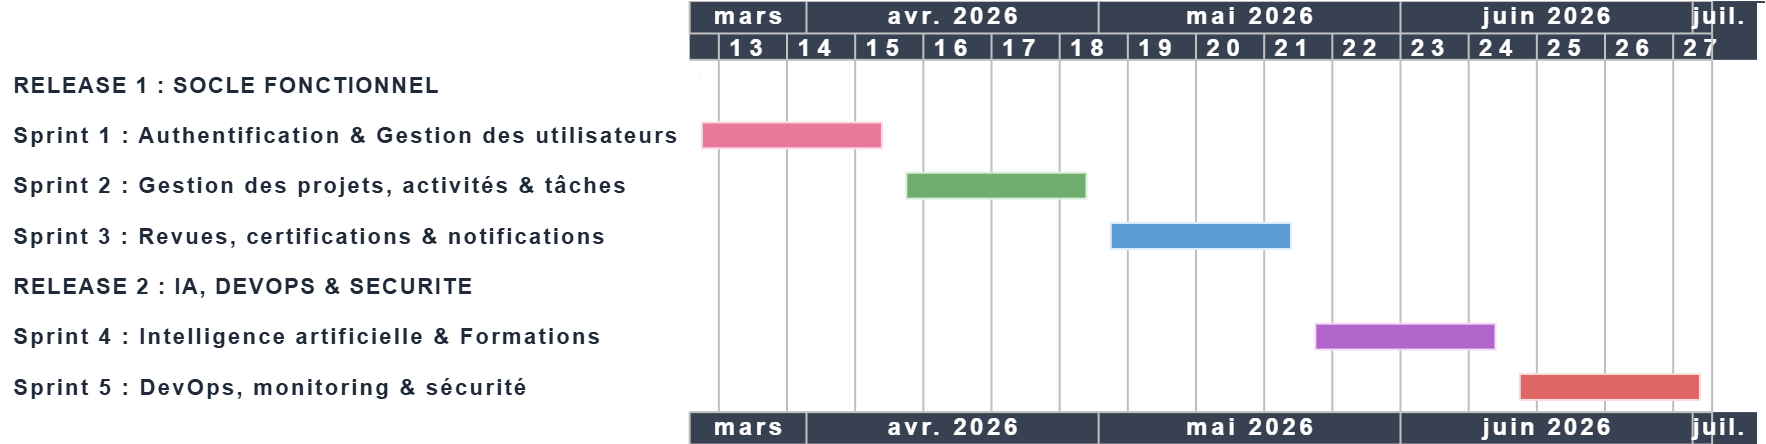
\includegraphics[width=\textwidth]{images/gantt.png}
  \caption{Planification globale des sprints (diagramme de Gantt)}
  \label{fig:gantt}
\end{figure}


% ─────────────────────────────────────────────────────────
\section{Architecture de la solution}
\label{sec:architecture}
% ─────────────────────────────────────────────────────────

\subsection{Architecture physique}

L'architecture physique de SmartPM repose sur un modèle \textbf{3-tiers}~\cite{arch3tiers} classique,
séparant la couche présentation, la couche métier et la couche données.

\begin{itemize}
  \item \textbf{Couche présentation :} Application Angular~19 (Single Page Application),
  servie par un conteneur Nginx exposé via le NodePort 30080 de Kubernetes.

  \item \textbf{Couche métier :} API REST développée avec NestJS, exposée via le
  NodePort~30000. Elle gère l'ensemble de la logique métier, l'authentification JWT,
  et la coordination avec les autres services.

  \item \textbf{Service IA :} Microservice FastAPI (Python) exposé via le NodePort~30800,
  responsable du chatbot contextuel et des simulations de projets.

  \item \textbf{Couche données :} MongoDB Atlas, base de données NoSQL hébergée en
  cloud, accessible depuis le cluster Kubernetes via une connexion sécurisée TLS.
\end{itemize}

\begin{figure}[H]
  \centering
  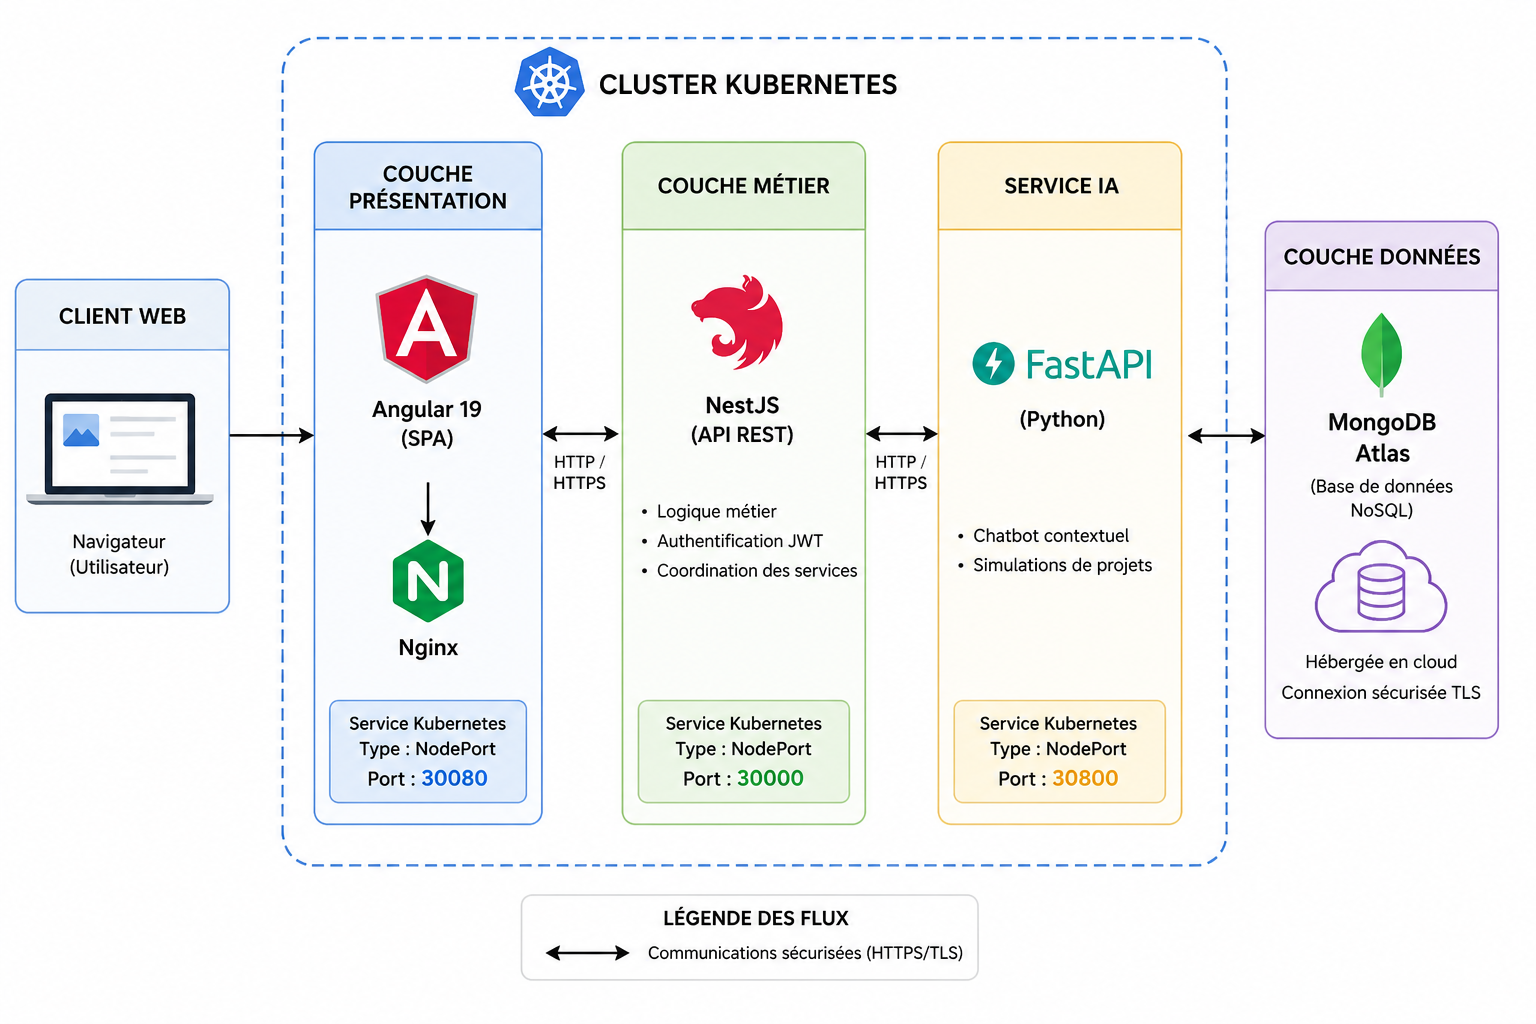
\includegraphics[width=0.9\textwidth]{images/architecture_physique.png}
  \caption{Architecture physique 3-tiers de SmartPM}
  \label{fig:archi_physique}
\end{figure}

\subsection{Architecture logicielle}

L'architecture logicielle de SmartPM suit le patron \textbf{MVC}~\cite{mvc} (Model-View-Controller)
côté backend, complété par une architecture modulaire propre à NestJS~\cite{nestjs}.

\begin{itemize}
  \item \textbf{Frontend (Angular 19)~\cite{angular} :} Architecture par composants avec services injectables
  pour la communication avec l'API. Chaque fonctionnalité est encapsulée dans un module Angular
  autonome (AuthModule, ProjectModule, AiChatbotModule...).

  \item \textbf{Backend (NestJS) :} Architecture modulaire avec séparation claire des
  responsabilités (Controller~$\rightarrow$ Service~$\rightarrow$ Schema Mongoose). Les modules
  indépendants sont : AuthModule, UserModule, ProjectModule, ActivityModule, SubActivityModule,
  TaskModule, ReviewModule, CertificationModule, NotificationModule, CommentModule,
  AiIntegrationModule, TrainingModule, AdminModule.

  \item \textbf{Service IA (FastAPI) :} Architecture orientée routes avec gestion asynchrone
  des requêtes et streaming SSE (Server-Sent Events) pour les réponses en temps réel.
\end{itemize}

\begin{figure}[H]
  \centering
  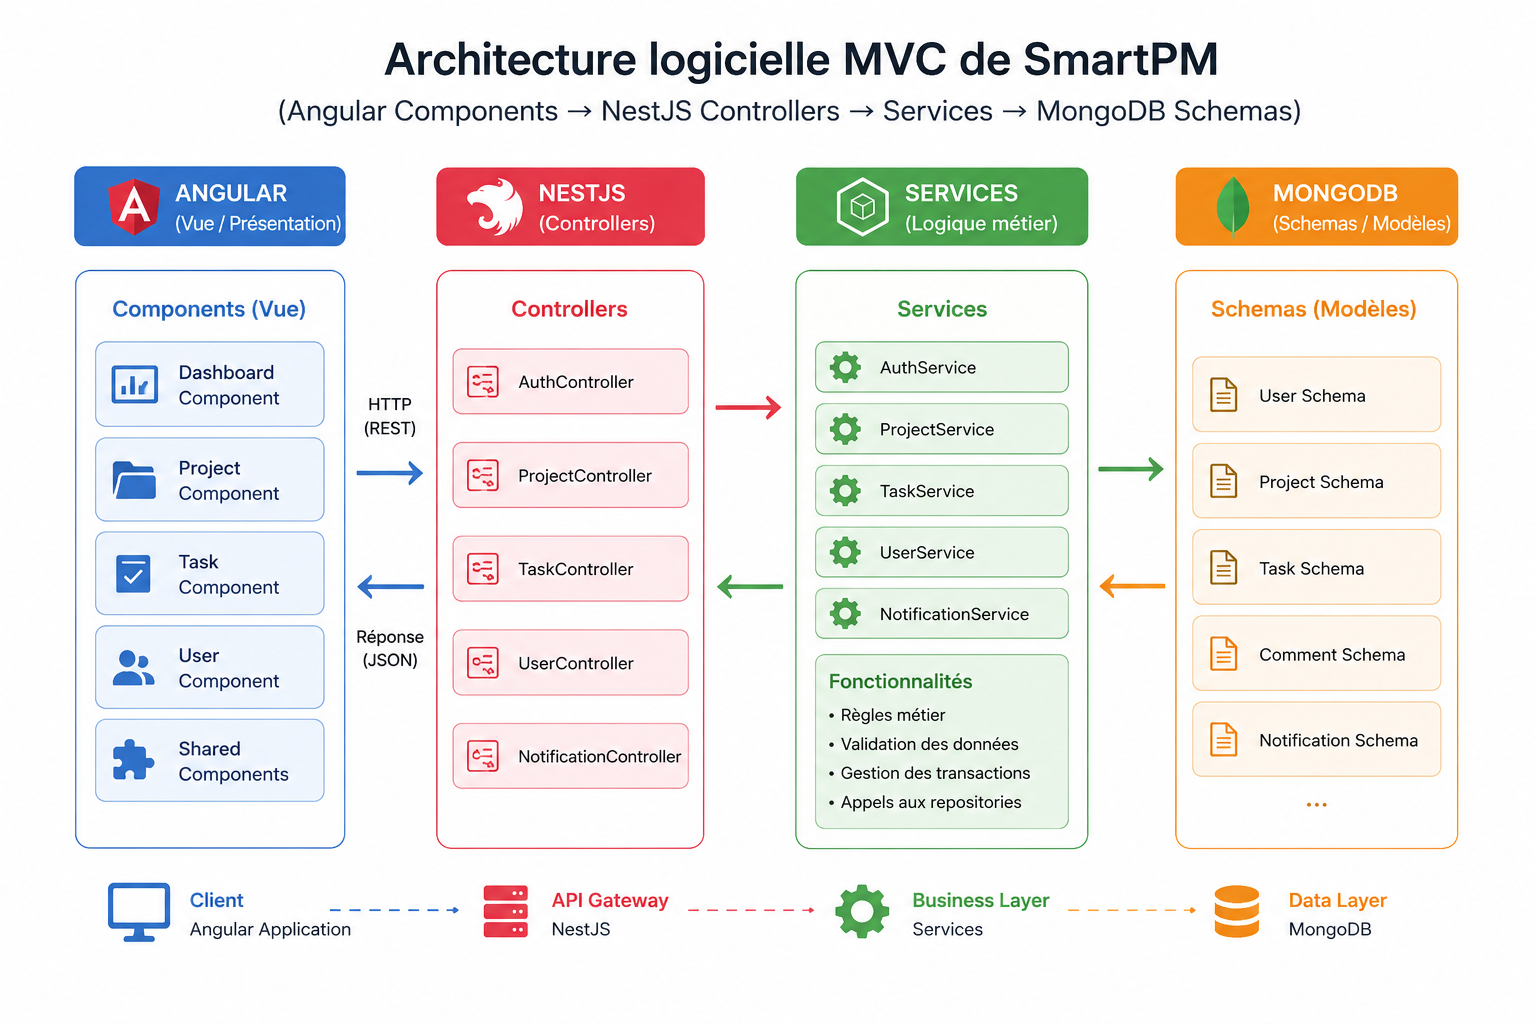
\includegraphics[width=0.85\textwidth]{images/architecture_logicielle.png}
  \caption{Architecture logicielle de SmartPM}
  \label{fig:archi_logicielle}
\end{figure}

\subsection{Architecture IA multi-modèles}

Le service IA de SmartPM est conçu selon une architecture \textbf{multi-LLM avec fallback},
garantissant la disponibilité du chatbot même en cas de saturation d'un fournisseur.

\begin{enumerate}
  \item \textbf{Groq (Llama 3.1-8b-instant)}~\cite{groq} — fournisseur principal, temps de réponse
  très court (approx 300ms Time-To-First-Token).
  \item \textbf{Gemini 2.5 Flash (Google)}~\cite{gemini} — premier fallback, haute qualité de réponse.
  \item \textbf{OpenRouter (Mistral 7B)}~\cite{openrouter} — second fallback, solution open-source.
\end{enumerate}

\begin{figure}[H]
  \centering
  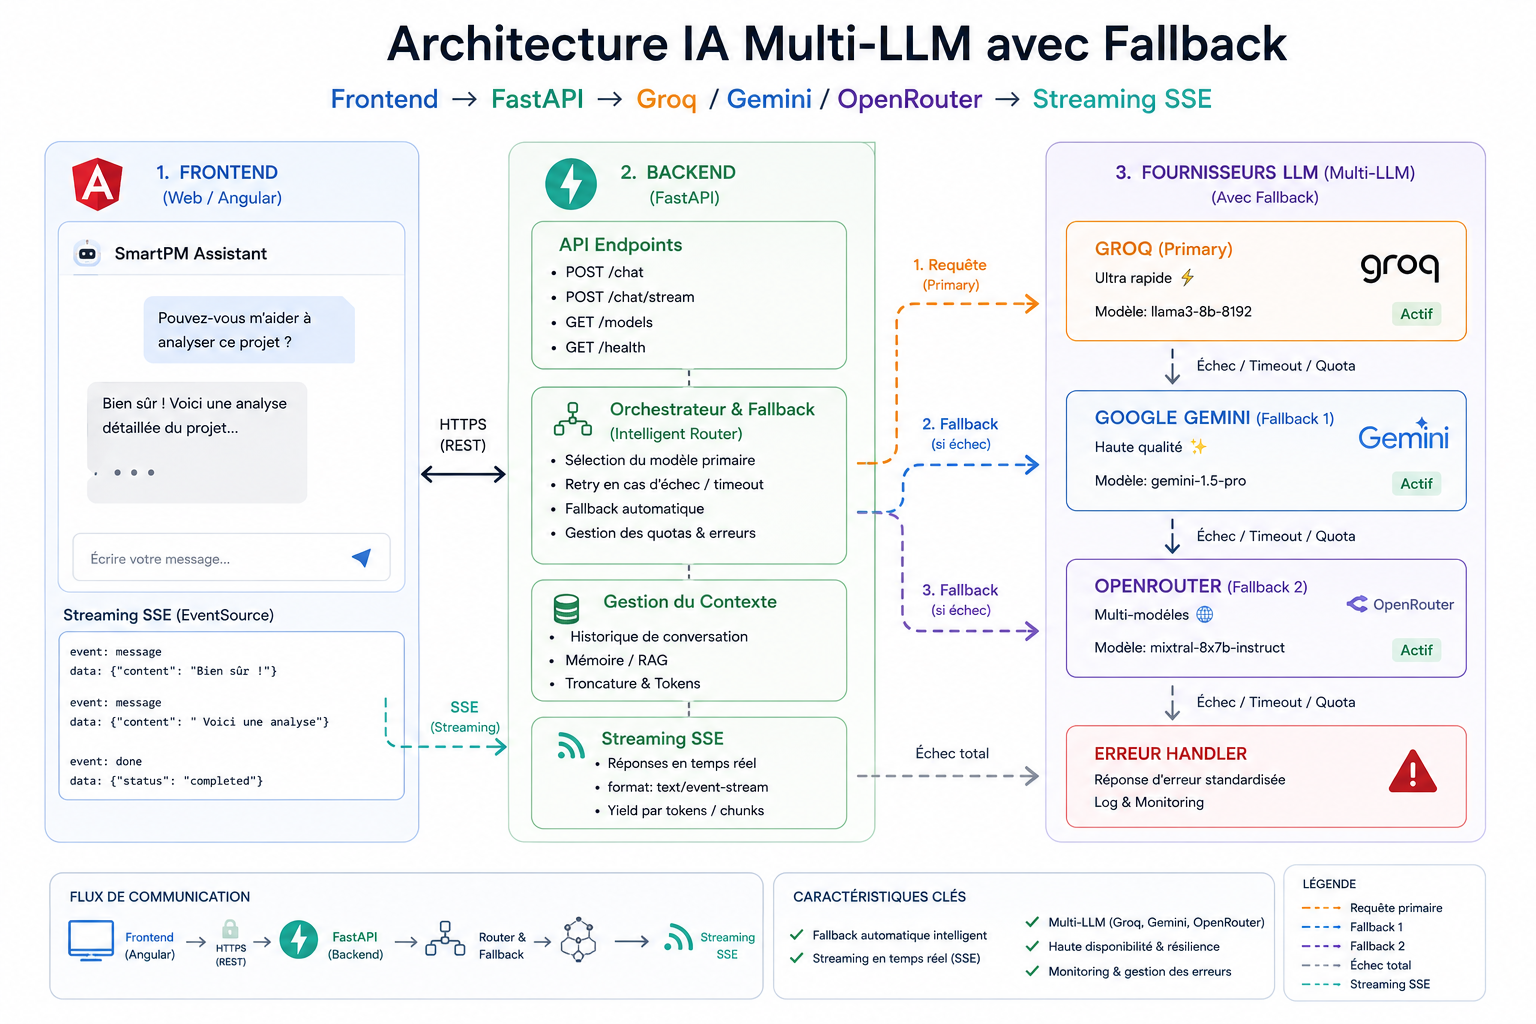
\includegraphics[width=0.8\textwidth]{images/architecture_ai.png}
  \caption{Architecture du système IA multi-modèles de SmartPM}
  \label{fig:archi_ai}
\end{figure}


% ─────────────────────────────────────────────────────────
\section{Choix techniques}
\label{sec:choix_techniques}
% ─────────────────────────────────────────────────────────

Le tableau~\ref{tab:choix_tech} récapitule les technologies retenues pour le développement
de SmartPM, accompagnées des justifications de chaque choix.

\begin{table}[H]
  \centering
  \caption{Tableau des choix techniques de SmartPM}
  \label{tab:choix_tech}
  \renewcommand{\arraystretch}{1.5}
  \begin{tabularx}{\textwidth}{|l|l|l|X|}
    \hline
    \rowcolor{tablehead}
    \textcolor{white}{\textbf{Couche}} &
    \textcolor{white}{\textbf{Technologie}} &
    \textcolor{white}{\textbf{Version}} &
    \textcolor{white}{\textbf{Justification}} \\
    \hline
    Frontend & Angular & 19 & SPA moderne, TypeScript strict, écosystème mature \\
    \hline
    Backend & NestJS & 11 & Architecture modulaire, decorators, JWT intégré, production-ready \\
    \hline
    Service IA & FastAPI & Python 3.11 & Asynchrone, SSE natif, excellent support LLM \\
    \hline
    Base de données & MongoDB Atlas & 7.0 & Flexibilité NoSQL, cloud natif, scalabilité horizontale \\
    \hline
    LLM Principal & Groq / Llama 3.1 & API & Rapidité $\approx$300ms TTFT, open-source, gratuit \\
    \hline
    LLM Fallback 1 & Gemini 2.5 Flash & API & Haute qualité, contexte large (1M tokens) \\
    \hline
    LLM Fallback 2 & OpenRouter / Mistral & API & Redondance, solution open-source \\
    \hline
    Conteneurisation & Docker & 26 & Portabilité, isolation, déploiement reproductible \\
    \hline
    Orchestration & Kubernetes & 1.30 & Scalabilité, haute disponibilité, rolling updates \\
    \hline
    Monitoring & Prometheus + Grafana & — & Métriques temps réel, dashboards visuels \\
    \hline
    Authentification & JWT + OAuth2 & — & Standard industrie, sécurité, stateless \\
    \hline
    Sécurité HTTP & Helmet + Throttler & — & Protection XSS, clickjacking, DDoS, brute-force \\
    \hline
    Proxy & Nginx & 1.25 & Serveur de fichiers statiques, performances élevées \\
    \hline
    Serveur Node & Node.js & 22 LTS & Runtime performant, non-bloquant, écosystème npm \\
    \hline
  \end{tabularx}
\end{table}


% ─────────────────────────────────────────────────────────
\section{Mise en place de la solution DevOps}
\label{sec:devops}
% ─────────────────────────────────────────────────────────

\subsection{Pipeline DevOps}

La solution DevOps de SmartPM repose sur un pipeline automatisé permettant de passer
du code source à un déploiement en production de manière reproductible et fiable.
Le pipeline se déroule en quatre étapes principales :

\begin{enumerate}
  \item \textbf{Build :} Construction des images Docker pour les trois services (Angular/Nginx,
  NestJS, FastAPI) à partir de Dockerfiles optimisés multi-stage.

  \item \textbf{Load :} Chargement des images dans le registre local de Minikube via la
  commande \texttt{minikube image load}, évitant la dépendance à un registre distant.

  \item \textbf{Deploy :} Application des manifestes Kubernetes (fichiers YAML) définissant
  les Deployments, Services, ConfigMaps et Secrets pour chacun des 6 pods.

  \item \textbf{Monitor :} Collecte automatique des métriques par Prometheus et visualisation
  dans Grafana, avec alertes configurables sur les seuils de performance.
\end{enumerate}

\begin{figure}[H]
  \centering
  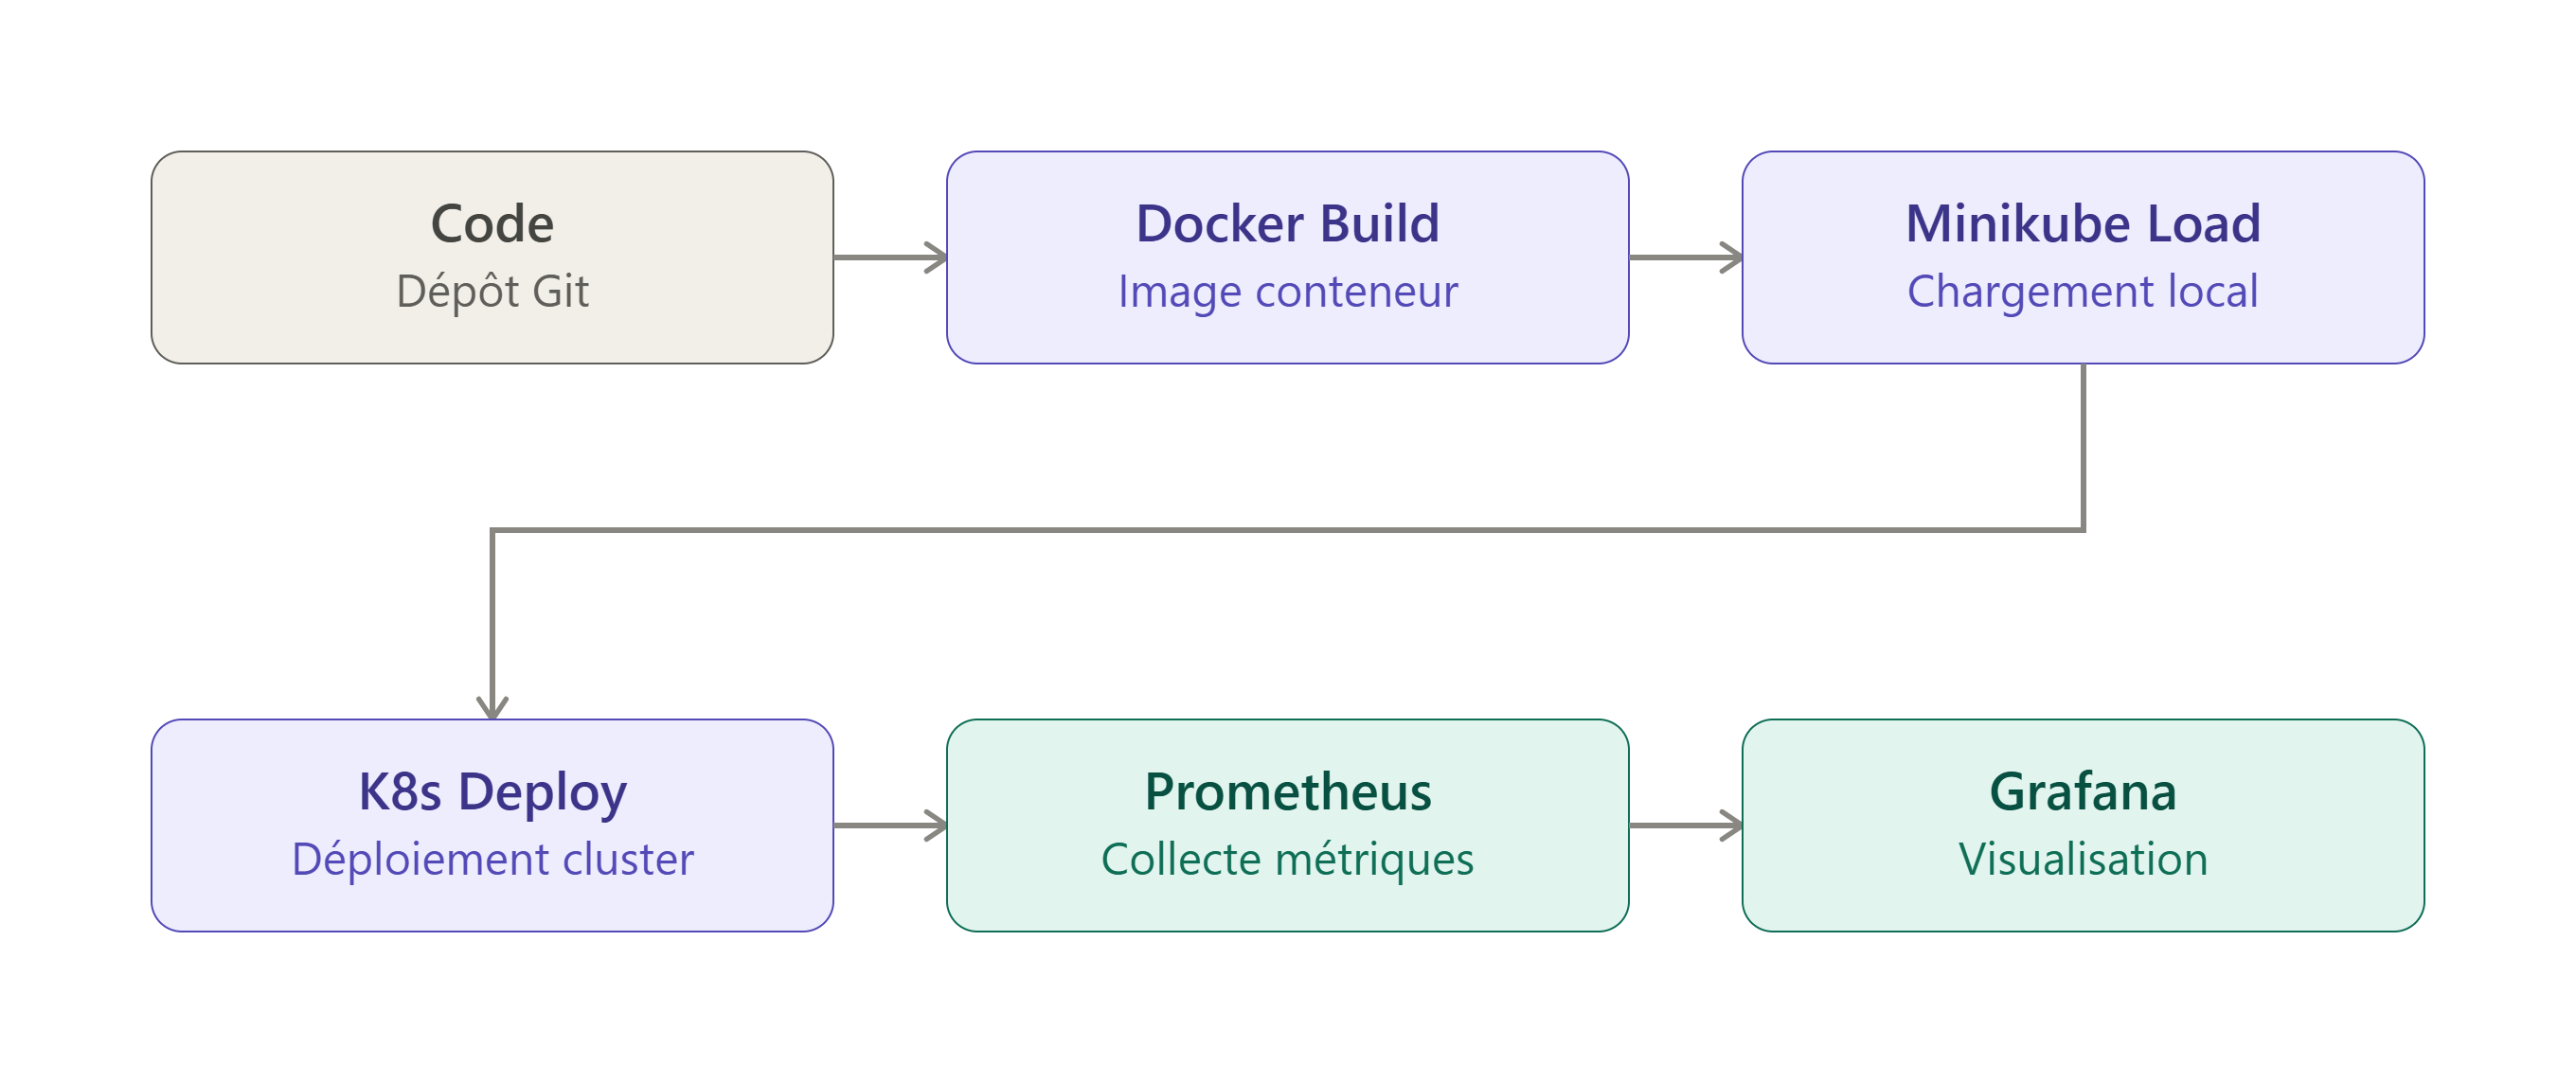
\includegraphics[width=\textwidth]{images/pipeline_devops.png}
  \caption{Pipeline DevOps de SmartPM}
  \label{fig:pipeline_devops}
\end{figure}

\subsection{Architecture Kubernetes}

Le cluster Kubernetes de SmartPM est composé de \textbf{6 deployments} interconnectés,
couvrant l'ensemble des besoins applicatifs et opérationnels de la plateforme.

\begin{table}[H]
  \centering
  \caption{Architecture Kubernetes — Pods et services de SmartPM}
  \label{tab:k8s}
  \renewcommand{\arraystretch}{1.4}
  \begin{tabularx}{\textwidth}{|l|l|l|X|}
    \hline
    \rowcolor{tablehead}
    \textcolor{white}{\textbf{Service}} &
    \textcolor{white}{\textbf{Image}} &
    \textcolor{white}{\textbf{NodePort}} &
    \textcolor{white}{\textbf{Rôle}} \\
    \hline
    Frontend & smartpm-frontend & 30080 & Interface Angular servie par Nginx \\
    \hline
    Backend & smartpm-backend & 30000 & API REST NestJS \\
    \hline
    AI Service & smartpm-ai & 30800 & Chatbot FastAPI + LLM streaming \\
    \hline
    MongoDB & mongo & — & Base de données (remplacé par Atlas en prod) \\
    \hline
    Prometheus & prom/prometheus & 30900 & Collecte de métriques \\
    \hline
    Grafana & grafana/grafana & 30300 & Dashboards de monitoring \\
    \hline
  \end{tabularx}
\end{table}

\begin{figure}[H]
  \centering
  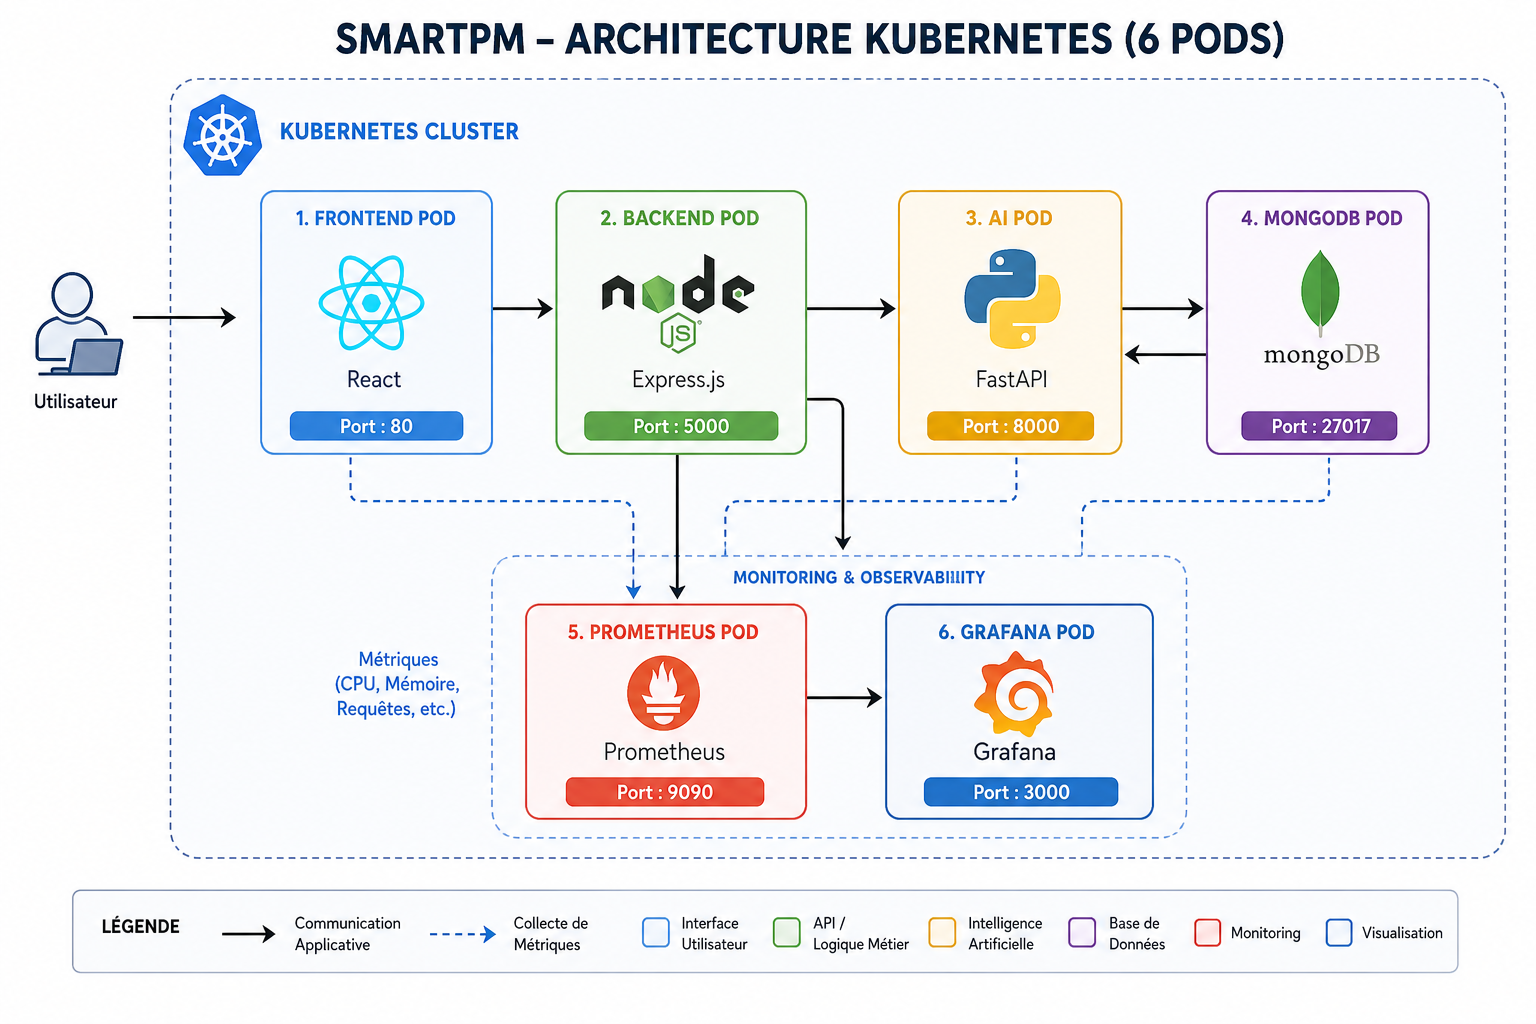
\includegraphics[width=\textwidth]{images/architecture_k8s.png}
  \caption{Architecture Kubernetes complète de SmartPM}
  \label{fig:archi_k8s}
\end{figure}


% ─────────────────────────────────────────────────────────
\section*{Conclusion}
% ─────────────────────────────────────────────────────────

Ce chapitre nous a permis de définir avec précision les besoins fonctionnels et non
fonctionnels de SmartPM, d'identifier les acteurs du système et de structurer le backlog
produit selon la méthodologie Scrum. Nous avons également présenté l'architecture technique
retenue — physique, logicielle et IA — ainsi que les choix technologiques justifiés et la
solution DevOps sur Kubernetes.

\vspace{0.3cm}

Le chapitre suivant sera consacré à la première release du projet, couvrant les sprints~1,
2 et~3, qui constituent le socle fonctionnel de la plateforme SmartPM.
